\documentclass[
  % -- opções da classe memoir --
  12pt,				% tamanho da fonte
  %openright,			% capítulos começam em pág ímpar (insere página vazia caso preciso)
  openany,
  %twoside,			% para impressão em verso e anverso. Oposto a oneside
  oneside,
  %titlepage,
  a4paper,			% tamanho do papel.
  % -- opções da classe abntex2 --
  %chapter=TITLE,		% títulos de capítulos convertidos em letras maiúsculas
  %section=TITLE,		% títulos de seções convertidos em letras maiúsculas
  %subsection=TITLE,	% títulos de subseções convertidos em letras maiúsculas
  %subsubsection=TITLE,% títulos de subsubseções convertidos em letras maiúsculas
  % -- opções do pacote babel --
  english,			% idioma adicional para hifenização
  brazil
]{article}
\usepackage[utf8]{inputenc}
\usepackage[brazil]{babel}
\usepackage{amsfonts}
\usepackage{indentfirst}
\usepackage[T1]{fontenc}
\usepackage{helvet}
\renewcommand{\familydefault}{\sfdefault}
\usepackage[left=3cm, right=2cm, top=3cm, bottom=2cm]{geometry}
\usepackage{setspace}
\usepackage{epigraph}
\usepackage{graphicx}
\usepackage{hyperref}
\usepackage{amsmath}
\numberwithin{figure}{section}
\numberwithin{table}{section}
\usepackage[raggedright]{titlesec}

%\usepackage{biblatex}
%\bibliography{relatorioEstagio}

\graphicspath{{figuras/}}

\renewcommand{\baselinestretch}{1.5}
\setlength{\parindent}{3em}
\setlength{\parskip}{1em}

%% DEFINEs dos textos constantes da capa
\newcommand{\defUFABC}{UNIVERSIDADE FEDERAL DO ABC}
\newcommand{\defBCC}{BACHARELADO EM CIÊNCIA DA COMPUTAÇÃO}
\newcommand{\defRelatorio}{RELATÓRIO DO ESTÁGIO SUPERVISIONADO III} %%ESTÁGIO SUPERVISIONADO
\newcommand{\defTitulo}{ESTÁGIO EM DESENVOLVIMENTO DE SISTEMA PARA USO INTERNO NA AGÊNCIA CADARIS E AGILE MASTER NO TIME DE ATENDIMENTO EDITORIAL DA FTD EDUCAÇÃO}
\newcommand{\defRafael}{RAFAEL CARDOSO DA SILVA}
\newcommand{\defOrientador}{Orientador: Prof. Dr. Daniel Morgato Martin}
\newcommand{\defLocaldata}{Santo André, 2019}

%%%%% \subsubsubsection
\usepackage{titlesec}
\usepackage{hyperref}
\titleclass{\subsubsubsection}{straight}[\subsection]

\newcounter{subsubsubsection}[subsubsection]
\renewcommand\thesubsubsubsection{\thesubsubsection.\arabic{subsubsubsection}}
\renewcommand\theparagraph{\thesubsubsubsection.\arabic{paragraph}} % optional; useful if paragraphs are to be numbered

\titleformat{\subsubsubsection}
{\normalfont\normalsize\bfseries}{\thesubsubsubsection}{1em}{}
\titlespacing*{\subsubsubsection}
{0pt}{3.25ex plus 1ex minus .2ex}{1.5ex plus .2ex}

\makeatletter
\renewcommand\paragraph{\@startsection{paragraph}{5}{\z@}%
  {3.25ex \@plus1ex \@minus.2ex}%
  {-1em}%
  {\normalfont\normalsize\bfseries}}
\renewcommand\subparagraph{\@startsection{subparagraph}{6}{\parindent}%
  {3.25ex \@plus1ex \@minus .2ex}%
  {-1em}%
  {\normalfont\normalsize\bfseries}}
\def\toclevel@subsubsubsection{4}
\def\toclevel@paragraph{5}
\def\toclevel@paragraph{6}
\def\l@subsubsubsection{\@dottedtocline{4}{7em}{4em}}
\def\l@paragraph{\@dottedtocline{5}{10em}{5em}}
\def\l@subparagraph{\@dottedtocline{6}{14em}{6em}}
\makeatother

\setcounter{secnumdepth}{4}
\setcounter{tocdepth}{4}



\begin{document}

%%--[ELEMENTOS PRÉ-TEXTUAIS]--%%

%%--CAPA--%%

\begin{titlepage}

\begin{center}
\text{ \defUFABC }
\text{ \defBCC }\\\vspace{5cm}
\textbf{\large{ \defRelatorio }}\\\vspace{3cm}
\textbf{\Large{\defTitulo}}\\\vspace{4cm}
% Nome do Autor
\textbf{\large{ \defRafael }}\\\vspace{1.5cm}
% Orientador
\textbf{\large{ \defOrientador }}\\\vspace{3cm}
\textbf{\defLocaldata}
\end{center}

\end{titlepage}

%%--FOLHA DE ROSTO--%%

\begin{titlepage}

\begin{center}
\textbf{\large{ \defRafael }}\\\vspace{5cm}
\textbf{\Large{ \defTitulo }}\\\vspace{5cm}
\begin{raggedleft}{
Relatório do Estágio apresentado ao Curso de\\
Bacharelado em Ciência da Computação como\\
requisito parcial para obtenção do grau de\\
Bacharel em Ciência da Computação
\\\vspace{1cm}

%  Trabalho apresentado à banca de Estágio\\
%  Supervisionado como requisito parcial para\\
%  obtenção do título de Bacharel em Ciência da\\
%  Computação pela Universidade Federal do ABC.\\
\large{ \defOrientador }
}\\\vspace{4cm}
\end{raggedleft}
\textbf{ \defLocaldata }
\end{center}

\end{titlepage}

%%--DEDICATÓRIA--%%

\begin{titlepage}

\begin{center}
\textbf{DEDICATÓRIA}
\end{center}

Dedico este trabalho realizado aos meus familiares e amigos que depositaram confiança desde o início para a realização deste meu projeto.

\end{titlepage}

%%--AGRADECIMENTOS--%%

\begin{titlepage}

\begin{center}
\textbf{AGRADECIMENTOS}
\end{center}

Aos meus pais pela confiança e apoio nas dificuldades enfrentadas durante todo o período da graduação.

Meus agradecimentos à agência Cadaris, principalmente a Diretora Comercial, que propôs essa oportunidade de alinhar meus conhecimentos obtidos na Universidade Federal do ABC no ambiente corporativo, além de crescimento pessoal e profissional.

Meus agradecimentos também à FTD Educação, principalmente ao Coordenador de Desenvolvimento, pela confiança a mim depositado para liderar o time e melhor atender as necessidades do Editorial.

A Ingrid Ferreira Costa pela paciência e força em sempre me ajudar a revisar este relatório.

\end{titlepage}

%%--EPÍGRAFE--%%

\begin{titlepage}
~\\\vspace{18cm}
\begin{raggedleft}

\begin{epigraph}
  {Aprendizado é isso: de repente, você compreende alguma coisa que sempre entendeu, mas de uma nova maneira.}
  {Doris May Lessing}
\end{epigraph}

\end{raggedleft}

\end{titlepage}

%%--RESUMO--%%

\begin{titlepage}

\begin{center}
  \textbf{RESUMO}
\end{center}

O presente relatório descreve as atividades realizadas durante o período de Estágio Curricular Obrigatório do Curso Superior de Bacharelado em Ciências da Computação oferecido pela UFABC - Universidade Federal do ABC. O objetivo geral do estágio consistiu no desenvolvimento completo de um sistema ERP (Planejamento dos Recursos da Empresa), da Proposta Comercial e de outros processos administrativos para a empresa Cadaris Comunicação.

A justificativa para o projeto é que o sistema atual contratado pela organização é ineficiente, desta forma, há necessidade do desenvolvimento de um novo sistema exclusivo que possa suportar os novos moldes da empresa, a fim de substituir esta ferramenta defasada. O novo sistema foi desenvolvido em PHP em conjunto com o \textit{framework} Laravel.

Iniciou-se o estágio com reuniões periódicas com a intenção de apresentar todas as regras de negócio da empresa e projetar o novo sistema para apoiar os processos administrativos. Após isso, houve o estudo necessário para a implementação do sistema, implantação e treinamento de seus usuários na empresa.

%TODO: update Resumo FTD
\end{titlepage}

%%--ABSTRACT--%%

\begin{titlepage}

\begin{center}
  \textbf{ABSTRACT}
\end{center}

This report describes how the developed activities during the period of Internship Required of the Computer Science Bachelor Course offered by UFABC - Federal University of ABC. The general objective of the internship consisted in the complete development of a ERP system (Enterprise Resource Planning), of the Commercial Proposal and other administrative processes, for the company Cadaris Comunicação.

The justification for the project is that the actual system hired by the organization is inefficient, thereby, there is a need of a new exclusive system that can be supported by the new molds of the company in order to replace this outdated tool. The new system was developed in PHP in conjunction with the Laravel framework.

It started the intership with periodic meetings with the intention of presenting all the company's business rules and design the new system to support the administrative processes. After this, there was the necessary study for the implementation of the system, deployment and training of its users in the company.

%TODO: update ABSTRACT FTD
\end{titlepage}


%%--LISTA DE FIGURAS--%%

\begin{titlepage}

\begin{singlespace}
  \listoffigures
\end{singlespace}

\end{titlepage}


%%-- LISTA DE ABREVIATURAS --%%



%%--SUMÁRIO--%%

\begin{titlepage}

\begin{singlespace}
  {\small
    \tableofcontents
  }
\end{singlespace}

\end{titlepage}


%%--[ELEMENTOS TEXTUAIS]--%%

\section{INTRODUÇÃO}

O estágio é uma atividade fundamental para a formação do aluno que está matriculado em um curso de nível superior, já que o discente tem a possibilidade de fazer uma aliança entre os conhecimentos adquiridos durante o período de graduação com a experiência vivencial no ambiente corporativo.

Além de agregar a responsabilidade de ter uma profissão, o estágio permite que o aluno desenvolva habilidades que são essenciais no mercado de trabalho, tais como liderança, trabalhar em equipe, resiliência, entre outros, através de situações e desafios que possam vir ocorrer dentro da organização e de suas responsabilidades.

O estágio é uma tarefa supervisionada por um orientador, e a descrição e avaliação do aluno quanto às suas atividades, conhecimentos adquiridos e habilidades desenvolvidas são relatados em um relatório.

Este relatório tem por objetivo descrever as atividades e os produtos obtidos durante a disciplina de Estágio Supervisionado em duas empresas. Nesta seção, apresenta-se a caracterização dos estágios, das empresas, uma visão geral do estágio e a organização geral deste documento.


\subsection{ESTÁGIO NA AGÊNCIA CADARIS}

\subsubsection{CARACTERÍSTICAS DO ESTÁGIO}

A modalidade deste estágio foi realizado em \textit{Home Office}\footnote{Escritório em casa, em uma tradução livre do inglês, trabalho que é realizado em espaço alternativo ao escritório de uma empresa.}, que também pode ser definido como um trabalho remoto ou teletrabalho. O estágio foi realizado na Cadaris Comunicação~\cite{cadaris}. A jornada de trabalho é de segunda à sexta-feira, desempenhando 6 horas diárias, totalizando 30 horas semanais, com a gratificação de uma bolsa de R\$ 1.100,00 por mês.

Por se tratar de um \textit{Home Office}, proporcionou ao discente um horário flexível de trabalho fazendo com que ele tenha autonomia para conciliar seu trabalho com as suas outras atividades. A comunicação com a empresa foi mantida através de e-mails e ligações via telefone e \textit{Skype}.

O objetivo geral deste estágio é o desenvolvimento de um projeto de uso interno para a empresa.


\subsubsection{CARACTERIZAÇÃO E ANÁLISE DA EMPRESA}

%  A Cadaris é uma agência de publicidade com atuação nas áreas de marketing, editorial e comunicação. Aqui, trabalho em equipe é lei e surpreender o cliente, uma meta diária.
%  Trabalhamos com ética e transparência, de forma responsável e comprometida. Produzimos com qualidade e criatividade, sempre com respeito aos prazos acordados.
%  Queremos ser reconhecidos como uma agência diferenciada, por clientes e funcionários.
%  Entre os nossos principais clientes estão: Colgate-Palmolive, Biotropic, ABO, TAM e Mattel, entre outras empresas.
%  Para saber mais sobre a Cadaris, acesse www.cadaris.com.br ou envie um email para cadaris@cadaris.com.br

%  Products:
%    Publicidade: anúncios, materiais de ponto de venda, materiais promocionais, apresentações de produtos e campanhas, hotsites, etc.
%    Comunicação: campanhas dirigidas e campanhas de comunicação interna
%    Editorial: revistas, informativos, enews, jornal-mural, guias e relatórios, manuais, cartilhas, etc.
%  ONDE A GENTE ATUA
%  EDITORIAL
%    Desenvolvimento de conteúdos editoriais baseado em planejamento, organização e processos de jornalismo.
%  ESTRATÉGIA
%    Criação de campanhas e peças de comunicação dirigida, comunicação interna, incentivo de vendas e marketing de relacionamento.
%  PUBLICIDADE
%    Assertividade em briefing, agilidade e criatividade são os drivers na criação das peças publicitárias e promocionais.
%  WEB
%    Levantamento de requisitos e necessidades, arquitetura da informação, design de projeto e desenvolvimento web.


O estágio foi iniciado no dia 01 de agosto de 2016 até dia 31 de maio de 2017, contratado pela Cadaris Comunicações, CNPJ 01.556.009/0001-46, que é uma agência de publicidade e está localizada na R. Dr. Thirso Martins, 100, cj 303, CEP:~04120-050, Vila Mariana, São Paulo~-~SP, telefone:~(11)~5571-9142.

Fundada em 11 de novembro de 1996, pelos sócios Maristela Harada e Frederico Pimenta, a Cadaris Comunicação é formada por profissionais de diferentes áreas da comunicação, o que proporciona mais eficácia e agilidade. Trabalhando com ética e transparência, de forma responsável e comprometida. Produzindo com qualidade e criatividade, sempre com respeito aos prazos acordados.

A Cadaris é uma agência de comunicação com atuação nas áreas de:
\vspace{-0.5cm}

\begin{description}
   \item [EDITORIAL] Desenvolvimento de conteúdos editoriais baseado em planejamento, organização e processos de jornalismo, como produtos: revistas, informativos, enews, jornal-mural, guias e relatórios, manuais, cartilhas, etc.
   \item [ESTRATÉGIA] Criação de campanhas e peças de comunicação dirigida, comunicação interna, incentivo de vendas e marketing de relacionamento.
   \item [PUBLICIDADE]  Assertividade em briefing, agilidade e criatividade, produzindo: Anúncios, materiais de ponto de venda, materiais promocionais, apresentações de produtos e campanhas, hotsites, e entre outros.
   \item [WEB] Levantamento de requisitos e necessidades, arquitetura da informação, design de projeto e desenvolvimento web.
\end{description}

Entre os principais clientes da Cadaris estão: Colgate-Palmolive, Biotropic, ABO, TAM e Mattel.


\subsubsection{VISÃO GERAL DO ESTÁGIO}

Durante o primeiro mês, o estagiário foi introduzido com o funcionamento da agência enfatizando a familiarização das regras do negócio e foi apresentado as ferramentas atuais utilizadas para apoiar a administração da empresa. A fim de desenvolver um \textit{software} de Sistema de Gestão Empresarial substituto para uso interno da Cadaris. 

Após este período, foi feito o estudo das tecnologias que seriam utilizadas para o desenvolvimento deste sistema proposto que já estavam sendo discutidas desde o início do estágio.

Em seguida, iniciou-se a implementação do sistema com foco inicial no \textit{Back-end} que foram seguidas em três etapas: Desenvolvimento do Cadastro de Recursos e algumas rotinas administrativas; Processo Comercial; Geração de Relatórios e Controle Financeiro.

Por fim, foi realizado a implantação do sistema em duas etapas, incluindo também o  treinamento de seus novos usuários e ajustes finais.



\subsection{EMPREGADO NA FTD EDUCAÇÃO}

\subsubsection{CARACTERÍSTICAS DO EMPREGO}

As atividades na empresa foram iniciadas com a contratação do discente como Pessoa Jurídica com o propósito de prestar serviços dentro das dependências da empresa que iniciaram a partir do dia 1 de junho de 2017. 

O cargo atribuído foi de Analista de Desenvolvimento Júnior, dentre as responsabilidades propostas, a principal, foi atender atender as demandas de programação \textit{Back-end} de novos componentes a serem integrados no sistema \textit{Controle de Projetos} (codinome \textit{Vulcano}) do Editorial da FTD.

%O \textit{Vulcano} é um sistema que mapeia os processos de diversos tipos de produtos digitais e físicos da FTD Educação e, com esse mapeamento, direciona as tarefas para cada um dos responsáveis.

%Todos os dias úteis, meio dia e meia noite, o sistema dispara um e-mail com as pendências que cada grupo de usuários deve resolver naquele momento. Ao resolver essa pendência, o projeto vai para o próximo grupo que precisa atuar até a sua conclusão.

Conforme a dedicação prestada e as habilidades desenvolvida do discente durante o desenvolvimento dos primeiros novos componentes, e por necessidade, foi formado um time para dar suporte exclusivo para o \textit{Vulcano}. Em que o discente se tornou o líder com a finalidade de conduzir um papel de metodologia ágil nesta equipe.

Posteriormente, foi contratado em regime de CLT para atuar no setor Editorial. Desenvolvendo atividades de liderança, participando efetivamente de reuniões de time, sendo responsável pela programação junto aos outros desenvolvedores da equipe a fim de compartilhar conhecimentos e revisar as realizações da equipe de trabalho.

O objetivo geral deste emprego é liderar a manutenção do \textit{Vulcano} e o desenvolvimento dos seus novos componentes.


\subsubsection{CARACTERIZAÇÃO E ANÁLISE DA EMPRESA}

% https://ftd.com.br/a-ftd/a-historia/
% https://pt.wikipedia.org/wiki/Editora_FTD

O vínculo empregatício na Editora FTD S/A iniciou-se no dia 5 de maio de 2018 e estende-se até atualmente. Empresa registrada pelo CNPJ: 61.186.490/0026-05, localizada na R. Manoel Dutra, 225, Bela Vista, São Paulo - SP, telefone: (11) 3596 – 6000.

Fundada em 1902 pelos Irmãos Maristas, a FTD é uma editora brasileira referência no mercado pela produção e oferta de soluções educacionais.

A nomeação ``FTD'' foi dada com o propósito de fazer uma homenagem a \textit{Frère Théophane Durand} que durante os anos de 1883 e 1907 esteve à frente da Congregação Marista como Superior Geral. Ele incentivou os Irmãos durante a sua gestão a escrever livros educacionais, obras que mais tarde vieram a pertencer a Coleção de Livros Didáticos FTD. Esse trabalho resultou em um enorme estímulo para a produção de mais obras didáticas e expansão deste negócio, marcando os Maristas como exemplos de educadores no nosso país~\cite{site_ftd}. 

Os valores da FTD sempre estiveram correlacionados com a sua missão de transformar a sociedade a partir do conteúdo educacional e cultural adequado e inovador, por isso é uma organização que valoriza o espírito de família entre seus colaboradores e clientes, amor ao trabalho durante o desenvolvimento das atividades, espiritualidade, justiça, presença significativa no mercado como forma de inspirar os colaboradores e clientes, e simplicidade para manter a transparência e autenticidade do trabalho desenvolvido~\cite{site_ftd}.

No século passado, a FTD foi a primeira editora de livros didáticos a cobrir todas as áreas de ensino. Além disto, grandes nomes da literatura tiveram suas primeiras obras publicadas pela editora, como por exemplo, Maurício de Sousa, referência da literatura infantil, que publicou os livros \textit{Piteco, Penadinho e Astronauta}~\cite{site_ftd}.

A FTD atua no mercado com os seguintes segmentos:

\begin{description}
	\item[LIVROS DIDÁTICOS] Produção de obras interdisciplinares de caráter pedagógico para serem utilizados em instituições de ensino. 
	\item[APOIO DIDÁTICO]   Produção de obras didáticas, pedagógicas e literárias, entre outros materiais de apoio à prática educativa de ensino formal e informal. 
	\item[LITERATURA]       Produção de obras literárias compostas por histórias fictícias ou não, no formato de poesia, em versos e em prosa. Classificados conforme sua escrita: romances, contos, artigos, ensaios, relatos jornalísticos, peças de teatro, histórias infantis, entre outros.
	\item[FTD DIGITAL]      A FTD oferece as suas obras em diferentes formatos digitais: PDFs, ePubs, LEDs, iBooks e Apps, com o propósito de facilitar a relação de jovens e adultos com os estudos e a literatura no geral. Além disto, oferece um ambiente online que permite que os alunos tenham acesso a provas e simulados para resolução, preparados pelos seus professores.
\end{description}


\subsubsection{VISÃO GERAL DO ESTÁGIO}

Este relatório contempla o período do desenvolvimento de um novo componente para apoiar as Pesquisas Iconográficas, uma etapa muito importante durante o desenvolvimento de um livro.

Foi iniciado realizando o levantamento de requisitos necessários a partir de uma entrevista com a Coordenadora da Iconográfia e o Coordenador do Fluxo Editorial. Na sequência, a equipe realizou o refinamento, planejamento, e por fim, o desenvolvimento do mesmo.

Sendo assim, este novo componente permitiu que todo o processo fosse realizado pelo \textit{Controle de Projetos} obtendo como resultado um grande ganho durante o gerenciamento de processos, já que anteriormente, esse trabalho era feito manualmente por planilhas e compartilhamento de arquivos via rede.


%\subsection{ORGANIZAÇÃO DESTE RELATÓRIO} %% {ORGANIZAÇÃO DO TRABALHO}
%
%As próximas seções estão organizadas como segue:
%
%A seção 2 apresenta as informações detalhadas de todas as atividades realizadas pelo estagiário. A seção está dividida em quatro partes, uma para cada atividade desenvolvida.
%
%A seção 3 descreve as considerações finais em relação a todo o estágio, como: contribuições para a formação, dificuldades encontradas e sugestões para trabalhos futuros.
%
%A seção 4 apresenta os principais problemas observados pelo estagiário em cada etapa e sugestões de melhorias para cada uma delas.
%
%A seção 5 detalha a relação entre as disciplinas cursadas pelo estagiário e as atividades realizadas durante os projetos.
%
%A seção 6 apresenta a conclusão sobre o estágio desenvolvido.


\clearpage
\section{ATIVIDADES DESENVOLVIDAS NA AGÊNCIA CADARIS}

%%--Descrever as atividades realizadas no estágio--%%

Esta seção tem como objetivo detalhar as atividades desenvolvidas durante o estágio supervisionado. Apresentando as atividades de aprendizagem; o desenvolvimento do projeto; e sua aplicação.

%  \noindent \texttt{Lista de trabalhos realizados:\\
%    ESTÁGIO 1 \\
%    - Reunião sobre as regras de negócio da empresa (DER) \\
%    - Estudo das tecnologias a serem utilizados (Laravel, bootstrap) \\
%    - Dev o sistema para substituir a antes utilizada (antigamente planilhas) \\
%    ESTÁGIO 2 \\
%    - Dev o sistema conforme as regras de negocio atual da empresa (software VBD) \\
%    - Dev o sistema para a geração de relatórios e controle financeiro \\
%    ESTÁGIO 3 \\
%    - Front-end (VueJS) \\
%    - teste, homologacao, e ajuste finais \\
%    - Outras áreas da empresa
%  }


\subsection{APRESENTAÇÃO DAS REGRAS DE NEGÓCIO}
\label{sec:2.1}

A administração de uma empresa é formada por diversos processos administrativos, que podem ser descritos em um conjunto de atividades que podem ser independentes e/ou relacionadas entre si, e que tem o papel de transformar todos os insumos advindos do trabalho em produtos e serviços que atendem as necessidades dos clientes e que são dotados de valor. Em apoio a cada processo são empregados diversas ferramentas tecnológicas. Entretanto, todas as empresas tendem a se evoluírem com o tempo, assim suas regras de negócio e seus processos evoluem juntos, e as suas ferramentas devem ser adaptadas ao novo modelo.

Em um dado momento na Cadaris, um software que apoia um dos seus principais processos administrativos, especificamente o de Propostas Comerciais, deixou de satisfazer as novas regras de negócio da empresa. Após inúmeras reclamações e \textit{feedbacks} da Cadaris ao proprietário do \textit{software} não serem corretamente atendidas. Então, foi decidido pelo desenvolvimento de um novo sistema exclusivo que possa suportar os novos moldes da empresa, a fim de substituir esta ferramenta defasada.

Portanto, o desenvolvimento deste novo sistema foi a principal responsabilidade dada neste estágio. Iniciando pela sua concepção e formalização, com o apoio de documentações como diagramas e modelos de processos.

O processo de Propostas Comerciais é realizado utilizando um sistema contratado desde 2013, este é instalado localmente em um servidor nas dependências da empresa para somente acesso local dos funcionários. O sistema foi desenvolvido em \textit{ASP}\footnote{ASP, abreviação para \textit{Active Server Pages}, também conhecido atualmente como ASP Clássico, é uma estrutura de bibliotecas básicas (e não uma linguagem) para processamento de linguagens de script no lado servidor para geração de conteúdo dinâmico na Web.} com integração ao banco de dados \textit{Microsoft SQL Server}\footnote{Sistema gerenciador de Banco de dados relacional desenvolvido pela Microsoft.}. E este apresenta muitos problemas, pois não se adapta aos novos padrões de desenvolvimento WEB, assim prejudicando, e muito, a experiência do usuário, por motivos que serão espanados a seguir.

Uma proposta comercial é iniciada com o contato do cliente para o setor de atendimento da Cadaris, no qual, o atendente irá realizar o cadastro de um \textit{job}\footnote{Trabalho, em inglês, trata-se do projeto a ser desenvolvido pela agência.}, preenchendo os dados necessários, em seguida é confeccionado o \textit{briefing}\footnote{O \textit{briefing} é um documento onde constam as informações do cliente com seus requisitos, a descrição do público-alvo e dos objetivos do cliente.} com um cronograma estimado sobre a produção deste \textit{job}. E por fim, o atendimento requisita um orçamento para o departamento responsável pelo financeiro da empresa.

Um funcionário do financeiro é encarregado de elaborar uma estimativa de custo para a realização deste \textit{job}. A estimativa é composta por dois tipos de custos: Internos e de Operacionalização. A estimativa de Custos Internos é montada com base em horas por tipo de serviço (Planejamento, Atendimento, Redação, Arte, Tráfego e Estratégia). A estimativa de Custos de Operacionalização refere-se à contratação de serviços de terceiros. Também é especificado o prazo e as condições de pagamento.

Logo após, é gerado um documento PDF\footnote{PDF (Portable Document Format) é um formato de arquivo, desenvolvido pela Adobe Systems para representar documentos de maneira independente do aplicativo.} com esta estimativa e outros dados importantes à respeito do orçamento em que é enviado para a diretoria comercial aprovar e assim retornar para o atendimento. Caso contrário, será devolvido para o financeiro para realizar as alterações exigidas pela diretoria.

Para concluir a etapa de Proposta Comercial, o atendimento retorna ao cliente com o orçamento para este ser aprovado por ele, a fim de dar início à produção do \textit{job}. Caso contrário, é solicitado alterações retornando para o \textit{briefing}, ou então o \textit{job} é arquivado se haver desistência do cliente em contratar a agência.

Pode-se ver na Figura a seguir, o modelo de processo da Proposta Comercial.

%\textbf{[[ img: modelo de processo Proposta Comercial (pagina em paisagem) ]]}
\begin{figure}[h]
  \centering
  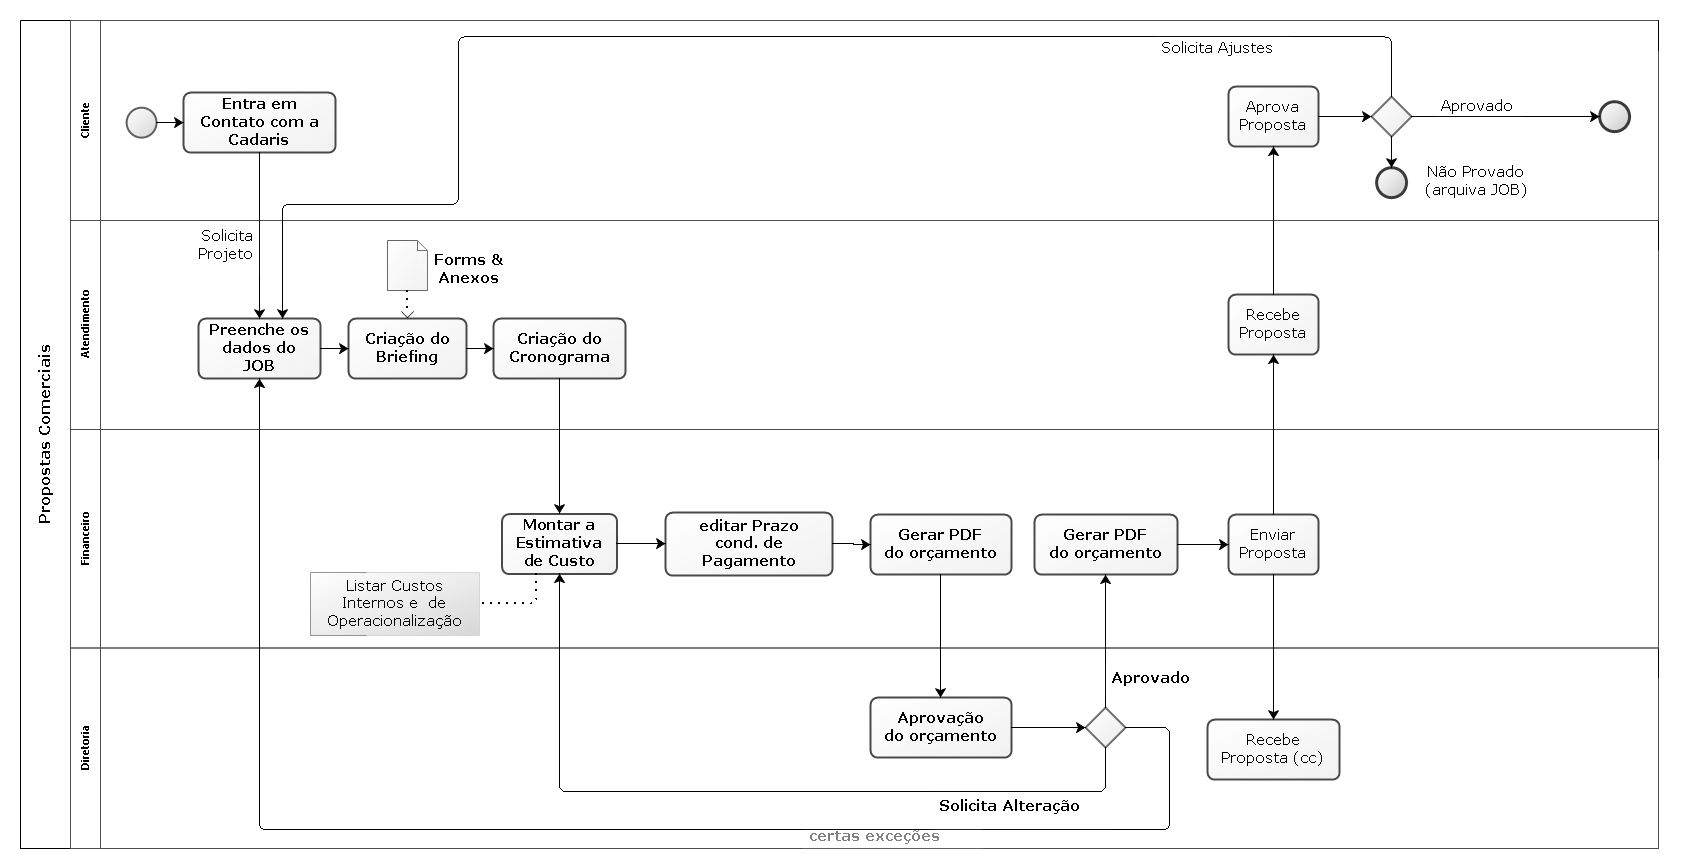
\includegraphics[width=\linewidth]{ModeloProcesso_Comercial_PeB}
  \caption{Modelo de Processo da Proposta Comercial}
  \label{fig:modProcess}
\end{figure}


A etapa de Produção do \textit{job} é realizado pelo setor de produção da Cadaris, utilizando técnicas e outras ferramentas especificas para o serviço desejado, como o \textit{Trello}\footnote{Ferramenta de gerenciamento de projetos em listas extremamente versátil, utilizando o método de \textit{Kanban} para indicar o andamento dos fluxos de produção.} para o gerenciamento do processo de produção. Concluido a produção do \textit{job}, o produto/serviço é entregue ao cliente. E para finalizar, o \textit{job} é encaminhado para o faturamento.

Também há outras rotinas administrativas que este projeto pretende abranger, já que são realizadas em um processo não automatizado, com o auxílio de planilhas eletrônicas:


{\singlespacing
\begin{itemize}
  \item Contas a receber;
  \item Contas a pagar;
  \item Controle RH:
  \begin{itemize}
    \item Folha de pagamento;
    \item Salário;
    \item Férias;
    \item Faltas/Atrasos;
    \item Folgas;
    \item Horas Extras;
    \item Vale Refeição;
    \item Vale Transporte;
  \end{itemize}
  \item Controle de Contratos;
  \item Cotação de Fornecedores;
  \item Relatórios:
  \begin{itemize}
    \item Relatório de Comissão;
    \item Relatório de Classificação de Receita;
    \item Relatório de Classificação de Despesa;
    \item Relatório Financeiro (Fluxo de Caixa);
  \end{itemize}
\end{itemize}
}


\subsubsection{PROBLEMAS ATUAIS E O PROJETO DE UM NOVO SISTEMA}
\label{sec:2.1.1}

Para compor a Proposta Comercial, este sistema contratado apresenta muitos problemas pelo qual os funcionários devem enfrentar. Resultando em empecilhos para a boa usabilidade e atrapalhando a performance do funcionário. Nesta seção será apontado defeitos do sistema atual e melhorias de recursos necessárias que o novo sistema deverá ter.

O sistema atual tenta ser generalista para suportar inúmeras áreas da empresa e agências com regras de negócio distintas. Assim, muitos de seus módulos se tornam ineficientes para atuar nos novos modelos de negócio, com muitos campos redundantes, ou sem funcionalidade, e não conta com operações automatizas. Um dos problemas mais comuns e sérios que ocorrem é que elementos importantes tem sua relação baseada na inserção manual de códigos identificadores para realizar a vinculação de um objeto a outro. Assim, de um ponto de vista da experiência do usuário, atrapalha a usabilidade do sistema e facilita o erro humano.

Para o preenchimento do \textit{Briefing}, além de um campo para a escrita livre, são necessários formulários especializados para os tipos de \textit{jobs} que a agência realiza, facilitando e padronizando a confecção destes \textit{Briefings}. O Cronograma é elaborado manualmente, então se faz necessário a incorporação de alguma ferramenta de simples utilização para a elaboração do cronograma estimado, pelo atendente para a realização do \textit{job}.

Para a transferência do \textit{job} cadastrado de um departamento para outro, durante a passagem das etapas, no sistema atual é necessário realizar um \textit{PIT}\footnote{Abreviação para Pedido Interno de Trabalho, é um documento com todas as informações necessárias para solicitar a realização de algum trabalho.}, que é livre para enviar para qualquer pessoa. Mas, visto que a Proposta Comercial da Cadaris segue uma ordem pré-estabelecida de etapas e departamentos envolvidos, então a adoção de um sistema mais especializado é uma ótima solução para agilizar o processo e impedir possíveis erros.

Já para a elaboração da estimativa de custo, em vários quesitos o sistema não atende corretamente ao modelo de negócio da Cadaris. Uma estimativa de custo contempla Custos Internos e Custos de Operacionalização que por sua vez é composto por listas de itens com seus respectivos valores, e para a elaboração desta lista de custos, além de campos desnecessários, há a falta de certas funcionalidades, tais como: maior personalização de taxamentos, arredondamento de valor, subcategorias de Tipo de Serviço no Custo Interno, valores padrão para cada Tipo de Serviço e outras funcionalidades.

O mais crítico do sistema é que essa estimativa de custo não é diretamente relacionada ao \textit{job}. Então, torna-se necessário preencher campos distintos com a mesma informação, pois o sistema não obtém esta informação do \textit{job} que deveria estar associado a ele. Algumas informações também importantes acabam sendo armazenadas em campos de observações por não ter campos próprios para aquela informação. E para finalizar, a estimativa não carrega as condições de pagamentos dos clientes, já que são distintas para cada um.

Ao final é gerado um documento em PDF contendo esta estimativa, porém faltam informações importantes neles como o prazo e condições de pagamento, e a lista de itens não são corretamente expostas. E no sistema atual este PDF da proposta pode ser gerado mesmo sem a aprovação da diretoria, havendo a necessidade de um bloqueio até a aprovação.

Durante todas estas etapas, é também utilizado no \textit{Trello} um \textit{card} para mostrar o estado do \textit{job}. Mostrando a necessidade de utilizar mais de uma ferramenta para gerenciar o processo de Proposta Comercial.

Para o gerenciamento de outros recursos, como: Funcionários, Departamentos, Clientes e Fornecedores, são utilizados planilhas eletrônicas. Sendo todo os processos relativos a estes recursos feito de modo não automatizado e sem uma centralização dos dados que são relacionados entre si.

Resumindo, a proposta geral deste projeto é o desenvolvimento de um sistema ERP\footnote{Abreviação em inglês para \textit{Enterprise Resource Planning}, ou seja, Planejamento dos Recursos da Empresa.}, que deve cuidar de todo o trabalho administrativo e operacional feito na Cadaris, e também automatizar todas estas tarefas antes feitas manualmente. Como por exemplo: faturamento, balanço contábil, fluxo de caixa, administração de pessoal, contas a receber, o dissídio, cálculo de férias e o ponto dos funcionários, e outros.

Há também um módulo especializado em atender a Proposta Comercial e todos os outros processos envolvidos nele.

Outros requisitos importantes são: o sistema deve ser de fácil acesso; possibilidade de utiliza-lo online e fora das dependências da empresa; garantir a disponibilidade; garantir a integridade, a segurança e a centralização de todos os dados; hierarquia de usuários; reduzir ao máximo o custo para desenvolvê-lo e mantê-lo ativo.



%  \noindent TODO: \\
%  - Explicar como eh o Comercial atual (VBD) OK \\
%  - dependeria de outros recursos (func client forn) q usa planilhas e códigos loucos OK \\
%  - automatizar tarefas/rotinas administrativas (ferias, horas, dissidio) OK \\
%  - producao (trello) OK \\
%  - finaceira (contas receber/pagar) OK \\
%  - integracao total dos dados, seguranca, divisao de usuarios e responsabilidades (hierarquia) OK \\




\subsection{ESTUDO DAS TECNOLOGIAS DE DESENVOLVIMENTO WEB}

Nesta subseção é relatada como ocorreu o estudo para a escolha de todas as tecnologias a serem empregadas no desenvolvimento deste sistema WEB, na qual muitas delas o aluno ainda não havia tido contato.

Como pode ser visto nas seções a diante, a UFABC oferece, por meio de disciplinas, todo o embasamento necessário para o desenvolvimento de um sistema, como: teoria da computação; concepção de um sistema de informação; modelamento de banco de dados; conceitos de interface gráfica; paradigmas de programação; programação para web e dispositivos móveis.

O mercado de trabalho necessita e busca sempre por praticidade, seguindo tendências de desenvolvimento e utilizando o que há de mais novo e eficiente no mercado. Atualmente, há diversos métodos e padrões de projetos que garantem eficiência de uma implementação. Além de inúmeras linguagens de programação, na qual nelas a massiva adoção de \textit{frameworks} para diversos fins.

Um \textit{framework} é um conjunto (ou biblioteca) de classes que se relacionam entre si para disponibilizar ao desenvolvedor funcionalidade especificas. Basicamente um \textit{kit} de ferramentas devidamente implementada, testadas e prontas para o uso. Poupando assim, tempo e trabalho do desenvolvedor de implementar operações básicas como acesso a banco de dados, sistema de templates, mapeamento de rotas, autenticação de usuário e validação de dados.

Com todos os requisitos discutidos anteriormente, escolher corretamente como será formada a arquitetura do sistema foi de total importância. Escolher uma linguagem de programação e com ela um de seus \textit{frameworks} disponíveis, determinará os requisitos mínimos para sua execução, como os custos para desenvolvê-lo e mantê-lo, e viabilizará todos os recursos requisitados. E também é relevante saber seus limites e a possibilidade de utilizar outras bibliotecas para apoiar a necessidade, assim então garantir o sucesso da implementação deste sistema web.

De início foi escolhido a linguagem \textit{PHP}, que será melhor explicada nas seções seguintes, como a linguagem para o \textit{Back-end}, onde será executada em um servidor, afim de servir páginas dinâmicas de \textit{HTML} ao cliente em um navegador de internet. A escolha desta linguagem dar-se pelo fato do discente já ter familiaridade com o desenvolvimento web utilizando \textit{PHP}.

A tarefa seguinte era a pesquisa e escolha de um \textit{framework} para apoiar o desenvolvimento. Após a leitura de blogs e artigos na internet sobre os melhores \textit{frameworks PHP}~\cite{top10}. Após pequenos testes e exames de projetos exemplos que utilizam o \textit{framework}, foi decidido pelo aluno que o \textit{framework} será o \textbf{LARAVEL}. Eleito como o mais popular por diversos sites, como o Sitepoint~\cite{sitepoint}, o Laravel foi lançado em 2011, mas apesar de ser relativamente novo, tem um enorme ecossistema, com uma ótima documentação e conteúdo didático na internet.

Para o aprender a utilizar o Laravel, o aluno estudou através de vídeo-aulas gratuitas disponíveis na plataforma \textit{LARACASTS}~\cite{laracast} e sempre consultando a documentação oficial~\cite{laraveldocs} Obtendo assim aptidão para criar aplicações web utilizando este \textit{framework}, conhecendo suas funcionalidades e recursos disponíveis.

Para então iniciar a implementação deste sistema ERP, relatadas nas próximas subseções.


\subsection{DESENVOLVIMENTO DO SISTEMA}

Após numerosas reuniões, com a Diretora Comercial e de Planejamento da Agência Cadaris e outros funcionários do departamento financeiro para apresentar e detalhar as necessitadas da empresa foi então iniciada a implementação do sistema. 

Como relatado anteriormente, o novo sistema visa dar total suporte ao processo de Propostas Comerciais, e também a administração Financeira da empresa, gerando Relatórios e controlando o Fluxo de Caixa. Mas inicialmente, foi necessário o desenvolvimento dos cadastros de todos os recursos da empresa, que se relacionarão com outras funcionalidades.


\subsubsection{CADASTROS}
Todo o gerenciamento de recursos da Cadaris eram feitas por planilhas eletrônicas, causando uma descentralização dos dados que se relacionam entre si, sem automatização de processos administrativos. Dificultando assim o trabalho dos funcionários e possibilitando erros.

Então, o primeiro desafio para o desenvolvimento deste sistema foi o levantamento de todos os recursos, separando-os em entidades e entendendo seus relacionamentos e atributos a serem armazenados. O Módulo de Cadastros devem concentrar todo os dados necessários para as funcionalidades desenvolvidas a diante.

A seguir é apresentado cada entidade e seus relacionamentos com os demais recursos do sistema. em todos há a funcionalidade de listar todos os itens, e também pesquisar por palavras, por valores em campos específicos e ordenar a lista de resultados com paginação. E é possível também criar um item, visualiza-lo, edita-lo e deleta-lo.


\subsubsubsection{Funcionários}

O primeiro cadastro a ser desenvolvido foi o gerenciamento de Funcionários. Neste deve contemplar a informação pessoal de cada funcionário e sua vida profissional dentro da Cadaris. 

Dentre suas informações pessoais esta seu: nome completo, sexo, e-mail, estado civil, CPF, RG, data de nascimento, nome do pai, nome da mãe, endereço atual, telefones de contato, dependentes, e informações bancárias.

Já nas informações profissional esta seu: teste MBTI\footnote{O teste MBTI, que significa Myers-Briggs Type Indicator (Classificação Tipológica Myers-Briggs), é um teste para classificar as características de uma pessoa.}, inativo, regime, horário de expediente, tempo de casa, cargo e nível, salário, Vale Refeição, Vale Transporte, Seguro de Vida e todos o histórico do funcionário.

O histórico do funcionário armazena os acontecimentos profissionais ordenados cronologicamente, e tais eventos são: contratação, mérito, dissídio, promoção, reajuste do vale refeição, reajuste do vale transporte, modificação do seguro de vida, aquisição de período aquisitivo e gozo de férias.

Algumas tarefas administrativas foram implementadas sobre este módulo, como a adição em lote de eventos no histórico dos funcionários para quando houver férias coletivas, por exemplo, calculo do valor de dissídio, e controle de pontos do banco de horas para gestão de faltas e horas extras. E ainda a visualização de alguns relatórios como: a férias acumulada e a faixa salarial de cada funcionário.


\subsubsubsection{Departamentos}

Todas empresas são subdivididas em departamentos, com suas próprias funções e organogramas, assim cada departamento desenvolve atividades e se inter-relaciona com outros departamentos.

Na Cadaris não é diferente, nela há departamentos que desempenham atividades especificas com profissionais especializados. Nela há os seguintes departamentos: Administração, Arte, Atendimento, Financeiro, Planejamento e Redação. E por meio do formulário do Cadastro do Funcionário é possível indicar qual Departamento o funcionário pertence.

E no sistema cada Funcionário está relacionado a um Departamento, pois será necessário para relacionar uma funcionalidade  do sistema para os funcionários de um departamento. Por exemplo, no Módulo Comercial cada Departamento desempenha uma função em cada etapa da elaboração de uma Proposta Comercial.


\subsubsubsection{Usuários}

Um dos itens mais importante de qualquer sistema são os seus usuários. O sistema foi todo pensado e projetado para melhor suportar as necessidades dos funcionários, que o utilizará para apoiar as suas atividades. Cada Usuário é necessariamente um Funcionário, assim ao cadastrar um novo Funcionário é possível cadastrar junto um Usuário para ele. E por meio do e-mail corporativo o funcionário recebe as instruções de acesso.

Assim em conjuntos com o Cadastro de Usuários, o sistema deve permitir o acesso do funcionário as funcionalidades do sistema por meio de um \textit{Login}. E também restringir o acesso a certas funcionalidades que não são da competência do tipo de funcionário em questão. Por meio de um seletor no formulário dos dados do usuário é possível escolher a sua alçada. Foram definidos os seguintes papéis para ser atribuído a cada Usuário: Administradors, Diretor, Funcionário do Financeiro, Funcionário do Planejamento, Funcionário doa Produção e Funcionário do RH.

Ao longo sistema há verificações de Permissões enraizadas nas funcionalidades, provendo total segurança para um funcionário não acessar dados que não são permitidos serem visualizados ou editados por ele.


\subsubsubsection{Clientes}

Os clientes são de suma importância para qualquer empresa, conhecê-los é crucial para melhorar a qualidade de seus produtos e serviços que são comercializados, isso permite criar uma relação duradoura que melhor atendam os objetivos de ambos os lados.% A Cadaris é uma agência de comunicação e tratar bem o cliente é essencial, e todos artifícios para melhor compreende-los se faz necessário. 

Na Cadaris seus Clientes são organizados numa forma de árvore hierárquica, isso porque a agência valoriza seus clientes de modo individualizado. O primeiro nível desta árvore é o conjunto de Empresas, o segundo nível são os Departamentos da Empresa e no terceiro, e último, nível trata-se dos Centros de Custos daquele Departamento. Conforme essa estrutura complexa, e por anteriormente a empresa já utilizar planilhas para armazenar cadastros, criou-se códigos definidos para indicar a hierarquia de cada item. Desta forma, o Cadastro dos Clientes deve manter essa estrutura e também os seus respectivos códigos, como exemplificado a seguir:

\vspace{-10mm}
\begin{singlespace}
	\begin{description}
		\itemsep0em 
		\item[$\bullet$~~~10] Empresa A
		\begin{description}
			\itemsep0em 
			\item[$\bullet$~~~10.01] Departamento A1
			\begin{description}
				\itemsep0em 
				\item[$\bullet$~~~10.01.01] Centro de Custo A1-a
				\item[$\bullet$~~~10.01.02] Centro de Custo A1-b
				\item[$\bullet$~~~10.01.03] Centro de Custo A1-c
			\end{description}
			\item[$\bullet$~~~10.02] Departamento A2
			\item[$\bullet$~~~10.03] Departamento A3
		\end{description}
		\item[$\bullet$~~~20] Empresa B
		\item[$\bullet$~~~30] Empresa C
	\end{description}
\end{singlespace}
\vspace{-5mm}

Na Empresa do Cliente é cadastrado todas suas unidades, e nestas Unidades há os seguintes dados: Nome Fantasia, Razão Social, CNPJ, Inscrição Estadual, Inscrição Municipal, Condição de Pagamento (utilizada no módulo Comercial), Informação Bancária e Endereço Completo.

No Departamento da Empresa é cadastrado a Lista de Contatos, na qual cada item é composto por Nome, Telefone, Celular e E-mail.

Dentro de cada Departamento é cadastrado o Centro de Custo sem dados adicionais. Deste modo, possibilita que cada \textit{Job} da Cadaris esteja associado à um Centro de Custo do seu Cliente, juntamente com os dados herdados dos itens anteriores auxiliando na formação da Proposta Comercial em que será entregue para o Cliente e executada pela Cadaris, como será relatado na seção \hyperref[sec:2.3.2]{2.3.2 - Comercial}.


\subsubsubsection{Fornecedores}

Os Fornecedores oferecem serviços, produtos e matérias-primas para apoiar todo e qualquer insumo da empresa, como por exemplo, telefonia, gráficas, confecção de brindes, servidores, \textit{freelancers}, e outros. Na Agência Cadaris, o cadastro de seus fornecedores e seu gerenciamento é substancial, já que contratar um fornecedor de qualidade irá garantir um trabalho mais satisfatório para seus clientes.

No sistema, Fornecedores possuem dois níveis e um código definido, semelhante aos Clientes. O primeiro nível é a empresa, na qual, são cadastrados os dados: CNPJ, Razão Social, Inscrição Estadual, Inscrição Municipal, Informações Bancárias, Classificação, Endereço Completo e Observações.

O item \textit{Classificação} é importante para avaliar a imagem do fornecedor dentro das seguintes atribuições: \textit{muito insatisfeito}; \textit{insatisfeito}; \textit{satisfeito}; e \textit{muito satisfeito}; assim como também pode atribuir uma \textit{nota geral}; \textit{nota de qualidade}; \textit{nota de atendimento}; e \textit{nota de prazo}; para ao final ter uma \textit{nota média}, além de observações e recomendações sobre este fornecedor.

O segundo nível trata-se dos produtos e serviços oferecidos pela empresa do fornecedor, formulário é cadastrado os contatos (como nome, telefone e e-mail) e \textit{Tags}, que auxiliam na realização de pesquisas, a fim dos funcionários realizarem cotações entre os produtos de seus fornecedores.

\subsubsubsection{Plano de Contas}

Plano de Contas é o conjutno de contas que guia os trabalhos contáveis da empresa, ela forma uma estrutura para a elaboração do \textit{Balanço Patrimonial}\footnote{O Balanço Patrimonial (BP) é um documento que relata a situação financeira de uma empresa considerando um período específico, geralmente um ano, levando em conta tanto fatores quantitativos como qualitativos.} e da \textit{Demonstração do Resultado do Exercício}\footnote{A Demonstração do Resultado do Exercício (DRE) é uma peça contábil que tem por objetivo detalhar a formação do resultado de um exercício (lucro ou prejuízo), por meio da comparação das receitas com os custos e despesas de uma empresa.}.

Cada item do Plano de Contas possui seu código e são agrupado em grupos. No Módulo Financeiro, cada despesa é relacionada a um item do Plano de Contas.


\subsubsubsection{Centros de Custo da Cadaris}

Centros de Custos da Cadaris tem a mesma finalidade do Plano de Contas, mas cadastrados separadamente, pois são utilizados em relações deferentes no Módulo Financeiro, que veremos a seguir.


\subsubsection{COMERCIAL}
\label{sec:2.3.2}
  
Nesta seção será apresentada os resultados da implementação do Módulo Comercial do Sistema, que compreende todas as regras de negócio expostas na seção \hyperref[sec:2.1]{2.1 - Apresentação das Regras de Negócio}.

Este módulo deve prover a sustentação de todo o processo de criação da Proposta Comercial, ilustrado pela \autoref{fig:modProcess}, utilizando os recursos cadastrados e contribuindo para o Módulo Financeiro. 

O Módulo Comercial foi subdividido em etapas, na qual em cada uma haverá interações exclusivas para cada tipo de funcionário e suas permissões de acesso. Em cada etapa é possível avançar a proposta comercial para a próxima etapa, salvar as alterações como rascunho e retroceder para a etapa anterior. 

O Usuário do tipo Administrador tem permissão para editar em todas as etapas e receberá notificação por e-mail em todos os casos.


\subsubsubsection{Criação da Proposta Comercial}

Para iniciar um \textit{Job} primeiro é criado a sua Proposta Comercial, na qual são preenchidos suas informações básicas, como: Nome da Proposta Comercial, o funcionário que a criou, a Unidade da Empresa do Cliente, o Centro de Custo do Cliente, uma breve descrição deste \textit{Job}, o Código da Receita, a data da previsão de entrega desta proposta, e a data e a hora da previsão da entrega do material deste \textit{Job}.

E somente o Funcionário do Financeiro e do Planejamento por criar uma Proposta Comercial. Em seguida é disparado um e-mail para o Funcionário do Financeiro avisando-os sobre um novo \textit{Job} que entrou na Etapa A.


\subsubsubsection{Etapa A - Confecção do Briefing e do Cronograma}

Nesta primeira etapa é confeccionado o \textit{Briefing} e o Cronograma da Proposta Comercial. O \textit{Briefing} trata-se das informações e instruções de como será o executado o \textit{Job}. O sistema possibilita para o usuário inserir o \textit{Briefing} por meio de cinco tipos de formulários:

\begin{description}
	\item[Livre] um editor de texto, que possui opções de formatações básicas para compor livremente todas as informações que desejar;
	
	\item[Cotação Gráfica] com o objetivo de compor informações pertinentes a materiais gráficos, como: medidas, tipo do material a ser impresso, acabamento, numero de páginas, tiragem, local de entrega, e outros;
	
	\item[Cotação Web] com o objetivo de compor informações pertinentes a materiais digitais para web, como: descrições, arquitetura de navegação, data para ir ao ar, pré-requisitos do servidor, domínio, tecnologias e linguagens envolvidas;
	
	\item[Cotação Brindes] com o objetivo de compor informações pertinentes a materiais ou objetos personalizados que serão utilizados como brindes, como: descrição, medidas, tipo de gravação, tiragem, referencias, local de entrega, e outros;
	
	\item[Anexos] conjunto de arquivos carregados no sistema a fim de contribuir com o \textit{briefing}, como por exemplo, materiais para referencia, artes gráficas, fotos, e outros.
\end{description}

Também nesta etapa é confeccionado um cronograma para a execução desta proposta comercial. Um diagrama de Gantt\footnote{O diagrama de Gantt é um gráfico usado para ilustrar o avanço das diferentes etapas de um projeto. Os intervalos de tempo representando o início e fim de cada fase aparecem como barras sobre o eixo horizontal do gráfico.} seria a melhor aplicação para este proposito, mas visto a sua grande complexidade, tanto de desenvolver um que atendar as requisitos, tanto de sua utilização pelos funcionários, foi utilizando um simples calendário em visão anual. Neste calendário é possível selecionar um período de dias e atribuir um evento para este período, com um departamento responsável e sua descrição. Atendendo de maneira mais simples e satisfatória os requisitos. 

Nesta etapa, somente tem permissão para editar o Diretor, o Funcionário do Financeiro e do Planejamento. E ao enviar esta proposta para a próxima etapa o Funcionário do Financeiro será avisado via e-mail.

\subsubsubsection{Etapa B - Orçamento e Condição de Pagamento}

Nesta etapa, o usuário poderá compor a Estimativa de Custo do \textit{Job} e cadastrar as condições de pagamento que será realizada pela cliente após a entrega do mesmo.

A composição da Estimativa de Custo é um estágio muito importante, ela é essencialmente a Proposta Comercial a ser entregue ao Cliente com a finalidade dele comprar o \textit{Job} da Agência. E também é umas das etapas mais criticadas no sistema anteriormente contratado pela agência, como foi discutida na seção ~\hyperref[sec:2.1.1]{2.1.1 - Problemas Atuais e o Projeto de um Novo Sistema}. Assim houve grande atenção ao projetar e desenvolver essa ferramenta de criação de Estimativas de Custo para atender eficientemente as necessidades da Cadaris.

Esta etapa possibilita a criação de inúmeras Estimativas de Custo para na etapa seguinte serem analisadas pela diretória. O formulário para confeccionar as estimativas são divididas em três níveis, em telas diferentes. A primeira tela tem-se a listas de todas as Estimativas de Custo deste \textit{Job}, possibilitando criar uma nova estimativa, editar-la, duplica-la, e duplicar a estimativa a partir de outra estimativa de um \textit{Job} diferente.

Editar uma estimativa, tem-se a segunda tela, na qual é listado os itens de Custo Interno da Agência e os Custos de Operacionalização relacionado a fornecedores. 

Nos itens de Custos Interno é possível adicionar itens, editar e excluir. Ao editar tem-se uma terceira tela que lista os itens de custo relacionado a Agência, como: arte, atendimento, planejamento, programação e redação. Cada item com seu valor unitário multiplicado pela quantidade de horas para a execução deste item. A soma deste itens teremos um subtotal, na qual será aplicado porcentagens de comissão e impostos. Neste calculo também é considerado um pedido da diretora, na qual ela quer que o valor final seja arredondado, assim ao subtotal é somado os centavos necessários para após o taxamento o valor final ser inteiro.

Nos itens de Custos de Operacionalização é possível adicionar itens, editar e excluir. Ao editar tem-se uma quarta tela que lista os itens de custo relacionado a fornecedores, na qual é possível selecionar o produto ou serviço dos Fornecedores cadastrados, é indicado o valor unitário e a quantidade para assim ter o valor do item, que serão somados em um subtotal, que será aplicado as porcentagens de taxamento, e também há o arrendondamento para estes itens.

A condição de pagamento é a descrição de como será pago pelo cliente o \textit{Job} realizado pela agência. Este formulário obtêm do cadastro do Cliente um valor padrão, visto que cada cliente trabalha de um modo e isso facilita para preencher este formulário.

Nesta etapa, somente tem permissão de editar o Diretor e o Funcionário do Financeiro. E ao avançar para a próxima etapa, o Diretor será avisado por e-mail.

Formado o assim as possíveis Estimativas de Custo deste \textit{Job}, que junto com a condição de pagamento, será repassado para a diretoria aprovar e ser encaminhado para o cliente nas próximas etapas.


\subsubsubsection{Etapa C - Aprovação do Diretor}

Nesta etapa, a diretoria deve revisar cada Estimativa de Custo confeccionadas anteriormente e avalia-las como: 

\begin{description}
	\item[Aprovada] estimativa aprovada poderá seguir à diante para ser oferecia ao cliente;
	\item[Não Aprovada] a estimativa deve ser ajustada e ser reavaliada novamente;
	\item[Reprovada] a estimativa não será oferecida ao cliente e será arquivada.
\end{description}

E com base nesta avaliação descidir se deve reotrnar para a etapa anterior ajustar ou seguir para a proxima etapa.

Nesta etapa somente o Diretor tem acesso, e ao retroceder para a etapa anterior, o Funcionário do Financeiro receberá uma notificação por e-mail, e se caso prosseguir para a próxima etapa o Diretor e o Funcionário do Planejamento serão notificados por e-mail.


\subsubsubsection{Etapa D - Geração do PDF e Aprovação do Cliente}

Mesta etapa, o Funcionário do Planejamento, que também faz o atendimento ao cliente, irá gerar um PDF para cada Estimativa de Custo, selecionando os Contatos cadastrados no Departamento do Cliente que irá receber a proposta, a Estimativa aprovada, e dentre os seguintes modelos de PDF:

\begin{itemize}
	\item Descrição geral e o Custos Internos;
	\item Descrição geral e o Custos de Operacionalização;
	\item Descrição geral e Custo Total;
	\item Descrição geral, Custos Interno e de Operacionalização e Custo Total;
	\item Descrição geral e Custos Interno e de Operacionalização;
\end{itemize}

O atendente entrega estas propostas para o cliente analisar se a agência será contratada. Se o Cliente aprovar, o funcionário indica na estimativa se ela foi aprovada, e seguirá para o próxima etapa. Se não for aprovada, voltará para o Etapa B para ser ajustada. Mas se a proposta for rejeitada, esta proposta inteira irá para uma etapa onde ficará arquivada.

Nesta etapa, somente o Funcionário do Planejamento tem permissão para editar, e ao encaminhar para a próxima etapa ou voltar para ajustes, o Diretor e Funcionário do Financeiro serão notificados por e-mail.


\subsubsubsection{Etapa E - Produção}

Após a aprovação do Cliente, a Proposta Comercial se torna um \textit{Job} para a agência, na qual será produzido conforme o modelo atual da empresa. E o sistema somente mostra nesta etapa as informações básicas, os \textit{briefings}, o cronograma, a estimativa de custo aprovadas.

Os Funcionário do Financeiro e do Planejamento tem permissão para acessar esta etapa e enviar este \textit{Job} para a próxima etapa, na qual o Diretor e o Funcionário do Financeiro serão notificados por e-mail.


\subsubsubsection{Etapa F - Faturamento}

Após o \textit{Job} ser finalizado e entregue ao cliente, ele se dirige para esta etapa, na qual ele será faturado, ou seja, a agência receberá o valor negociado na Proposta Comercial. E utiliza as Estimativas de Custo aprovadas para gerenciar este recebimento no Módulo Financeiro de Contas a Receber, que será melhor descrito nas seções subsequentes. 

O Funcionário do Financeiro tema acesso a esta etapa. Ao finalizar o faturamento, o \textit{Job} é enviado para a \textbf{Etapa G - Finalizado}, na qual agrupa todos os \textit{Jobs} concluídos, e o Diretor, o Funcionário do Financeiro e da Produção são notificados via e-mail. 

Há também outra etapa chamada \textbf{Etapa Z - Arquivado}, que persiste as Propostas Comerciais que foram rejeitadas, mas possibilita serem resgatados para voltarem para o início.

Atendendo todos os requisitos necessário e descrito pelo diagrama do modelo de processo ilustrado na \autoref{fig:modProcess}, que foram amplamente debatido e projetado junto com a sócia-diretora da Agência Cadaris para melhor atender suas especificidades.



\subsubsection{RELATÓRIOS E CONTROLE FINANCEIRO}

Nesta seção será descrito o Módulo Financeiro do Sistema desenvolvido. Controlar o financeiro da empresa é fundamental para manter saudável o equilíbrio do caixa, ajudar na gestão e no planejamento. Utilizar um sistema informatizado é a melhor solução para gerenciar e supervisionar todos os fluxos dos caixas, contas a pagar, contas a receber, e folhas de pagamento.

Em todos os componentes do Financeiro, somente tem acesso o Administrador, o Diretor e o Funcionário do Financeiro. Nas subseções seguintes será apresentado cada componente do Financeiro.


\subsubsubsection{Contas Bancárias}

Inicialmente é cadastrado as Contas Bancárias da empresa e seu valor inicial naquela data para a partir desta data o sistema irá calcular todos os fluxo de entradas e saídas desta conta.

Todo este módulo financeiro visa ser o mais flexível e abrangente para apoiar todos as atividades envolvidas na gestão da empresa. Uma das possibilidade é haver contas de investimento, que rendem com o tempo, entrando valores para a conta. Então, um componente para registar os rendimentos é conveniente. Nele é possível cadastrar o valor do rendimento, o impostos a serem recolhidos, a data e apontar qual a conta que será creditada o valor líquido.

É possível também haver transferências monetárias entre estas contas bancárias cadastradas. Então tem disponível um formulário para o registro desta transação, na qual o usuário informa a data, a conta bancária de origem, a conta bancária de destino, o valor bruto e a taxa a ser debitada pelo envio na conta de origem.

Assim como será detalhado mais a diante, o fluxo de caixa cuidará de gerenciar todas as entradas e saídas destas contas bancárias cadastradas.


\subsubsubsection{Contas a Receber}

Após a conclusão do \textit{Job}, a Cadaris deve receber o pagamento pelo serviço realizado. Buscando um ótimo relacionamento com seus clientes, tem-se a necessidade do sistema possibilitar grande flexibilidade com esses pagamentos. 

A partir do valor das Propostas Comercias contatadas, o Sistema possibilita o parcelamento deste valor em datas e valores configuráveis. O Funcionário do Financeiro entra no componente de Faturamento de Jobs, na qual sua primeira tela é a listagem de todos os \textit{Jobs} que estão na etapa de faturamento indicada lá no Módulo Comercial. Ao selecionar um \textit{Job}, entra-se na sua lista de parcelas, e o funcionário irá inserir parcelas que totalizam o valor total da proposta. 

Além de poder inserir manualmente o valor e a data de uma parcela para a conveniência do usuário, nesta tela possibilita a inserção de parcelas na qual o valor é uma porcentagem do valor total. Por exemplo, pode-se inserir uma parcela de 40\% e outra parcela de 60\% do valor total.

Em cada parcela é cadastrado a data de pagamento, a conta bancária que receberá o valor no fluxo de caixa, o valor bruto, o valor retido, valor líquido, a nota fiscal e a data de sua emissão.

Deste modo o sistema gerencia todas as contas a receber e pelo fluxo do caixa é possível acompanhar as entradas dos valores em suas datas.


\subsubsubsection{Contas a Pagar}

O Sistema também prove controle nas contas a serem pagas, que como os produtos e serviços contratados com fornecedores para apoio o \textit{Job}, ou contas de consumo da própria empresa.

Pada adicionar uma conta de fornecedor, é necessário indicar num formulário: o fornecedor,  a data de pagamento, a conta bancária, o centro de custo da Cadaris, o valor e anexar a nota fiscal e o comprovante. Ao ela ser paga, será indicado no Fluxo de Caixa a saída deste valor.

Para adicionar uma conta de consumo, é necessário indicar num formulário: a data de pagamento, a conta bancária, o centro de custo da Cadaris, a frequência desta conta, forma de pagamento, código de despesa, o valor e anexar a nota fiscal e o comprovante. Ao ela ser paga, será indicado no Fluxo de Caixa a saída deste valor.


\subsubsubsection{Folhas de Pagamento}

Outra rotina financeira muito importante em todas empresas é a folha de pagamento de seus funcionários. O Sistema deve prover automatização desta grande demanda que ocorre todos mês em um período.

No cadastro de um funcionário é indicado o seu histórico na Cadaris, na qual está cadastrado o seu salário, vale refeição e vale transporte acordado. Deste modo é possível calcular o valor que aquele funcionário deve receber da empresa.

O Funcionário do Financeiro acessa o Modulo de Folhas de Pagamento, na qual é possivel listar os salários lançados anteriores. Para lançar uma nova folha de pagamento com todos os funcionários ativos da empresa, basta somente clicar um botão e preencher qual o período referente e a data que será paga, que o sistema fará todo o calculo em lote do salários deles. Tornando-se muito rápido e prático para o Funcionário, evitando erros humanos.

Além do salário, o Sistema deve lançar o Pagamento de Férias do seus funcionários, basta o Funcionário do Financeiro adicionar um laçamento de férias, indicando em um formulário: qual o funcionário, número de dias, a data de inicio e ter minio, a data de pagamento, a conta bancária, o centro de custo da Cadaris, o valor do salário mensal, o valor das férias, o valor do acréscimo, o valor retido, o valor líquido e o valor do bruto.

Outro item que deve entrar na fluxo de saída é a Rescisão de um funcionário, neste formulário de cadastro é necessário: indicar o funcionário, a data de pagamento, a conta bancária, o centro de custo da Cadaris, o salário dos dias trabalhado, a hora extra, o DSR do salário, as férias, o terço de férias, a férias proporcionais, a férias paga, o aviso prévio, o 13º salário, o 13º salário proporcional, o previdência, a previdência do 13º salário, o INSS das férias, o desconto vale refeição e o desconto vale transporte.

Outra saída é a retirado de Sócios, na qual um sócio pode retira um montante da conta da empresa para si, semelhante a sua comissão. Num formulário basta indicar o sócio, a data de pagamento, a conta bancária, o centro de custo da Cadaris e a forma de pagamento.

O último item é o 13º Salário, que acontece a saída junto com a Folha de Pagamento, mas em duas parcelas ao final do ano. Somente é necessário indicar o funcionário, a data de pagamento, a conta bancária, o centro de custo da cadaris, o valor do 13º salário e o valor de desconto.


\subsubsubsection{Fluxo de Caixa}


Por intermédio dos cadastros de entradas e saídas, o Sistema deve calcular todo o Fluxo de Caixa ocorrido, por esse é o módulo mais importante do financeiro, pois é nele que fica registrado todo o cruzamento dos dados cadastrados e a demonstração do fluxo do caixa por completo em um certo período.

A primeira tela é um calendário em que é possível selecionar o período, na tela seguinte é escolhido a Conta Bancária, assim o sistema retorna à todas atividades registradas da conta e neste período especificado.

Na visualização do Fluxo de Caixa é separado em três seções. A primeira seção fica registrado as Contas a Receber onde constam em subseções a listagem de Faturamento dos Jobs, a Entrada de Transferências e o Rendimentos de Investimentos. Na segunda seção está registrado as Contas à Pagar, na qual suas subseções listam as Contas de Consumo, as Contas dos Fornecedores, a Saída de Transferências, a Folha de Pagamento, o Pagamento de Férias, a Retirada de Sócios, a Rescisão e o 13º Salários. Ao final de cada listagem é exibidor o seu subtotal, que é a soma simples dos itens que tiveram seus pagamentos efetuados, e o subtotal projetado, que é a soma simples de todos os itens pagos e com pagamento pendente. Por fim, na terceira seção é exibido o valor inicial deste período, a soma de todos os subtotais de saída, a soma de todos os subtotais de entrada, e finalmente, o saldo final deste período juntamente com a sua projeção.

Na listagem de cada item consta um indicativo dinâmico que muda a cor de fundo da linha para indicar se o pagamento do item está atrasado e quais são os item que vencem nesse dia. Deste modo, auxilia o usuário a identificar os itens importantes no momento de supervisionar o fluxo de caixa.

O registo completo deste fluxo pode ser exportado para uma planilha que lista todas as atividades neste período unificado de forma cronológica, possibilitando utilizar esses dados em filtros para extrair relatórios.



\subsection{PROVISIONAMENTO}

Nas seções anteriores foram descritos os componentes do sistema, mas o provisionamento deste tem grande importância também. O sistema foi hospedado em um \textit{Amazon Elastic Compute Cloud} da \textit{Amazon Web Services} que é uma plataforma de computação em nuvem, que permite rodar qualquer aplicação diretamente em computadores virtuais com uma instância de configuração básicas para suportar o sistema.

Na máquina virtual foi aplicada uma solução de contêineres com \textit{Docker}, provendo uma camada de abstração para automatizar a implantação em qualquer hospedagem. Deste modo, facilita uma rápida e automatizada configuração de todos os requisitos do sistema, como: PHP-FPM 7.0, MySQL, Nginx, \textit{daemon} para fila de execução assíncrona, e outros.

O sistema realiza \textit{backups} do banco de dados duas vezes ao dia, pois em caso de falha, os contêineres do \textit{Docker} facilitarão a fácil reconfiguração do provisionamento para que em menos de cinco minutos o sistema volte a estar \textit{online} com os dados restaurados. Com essa infraestrutura o sistema está bem condicionado para seu correto funcionamento e uma ótima performance .


\subsection{ENTREGA DO SISTEMA}

O Sistema foi entregue em duas fases, a primeira foi no termino o Módulo Comercial, conforme a necessidade de substituir o sistema contratado anteriormente, iniciando o seu uso pelo cadastro de todos os seus recursos e \textit{Jobs} feitos a partir no início do ano de 2017.

A segunda entrega foi na finalização do Módulo Financeiro, possibilitando a migração dos dados financeiros de todas as contas pagas e recebidas desde o inicio do ano de 2017. E também a necessidade de adicionar novos componentes antes não ponderado, como a Rescisão e o 13º Salário. 

Todo desenvolvimento do projeto foi acompanhado pela diretora para validar e homologar funcionalidades, indicando as alterações e as melhorias necessárias. A utilização do Sistema foi de fácil adaptação e aprendizado por toda equipe, as ferramentas de trabalho e os dados necessários para realizar certas ações foram otimizados com relação ao sistema que era utilizado anteriormente.

O Sistema foi muito bem recebido, pois demonstrou sua grande eficiência logo no inicio, quando houve a inserção de todo o histórico de transações no Módulo Financeiro, ao ponto dos valores calculado pelo sistema se tornarem síncronos com as Contas Bancárias reais da empresa.






\clearpage
\section{ATIVIDADES DESENVOLVIDAS NA FTD EDUCAÇÃO}

\subsection{PRODUTOS DA FTD}
\subsubsection{METODOLOGIA ÁGIL NA FTD}

\subsection{SOBRE O CONTROLE DE PROJETOS}
\subsubsection{FERRAMENTAS DO VULCANO}

\subsection{DESENVOLVIMENTO DO ICONR}
\subsubsection{\textit{GROOMING}}
\subsubsection{\textit{PLANNING}}
\subsubsection{DESENVOLVIMENTO}
\subsubsection{\textit{REVIEW}}






\clearpage
\section{FUNDAMENTAÇÃO TEÓRICA}

%%-- Descrever as disciplinas utilizadas e dar exemplos--%%

Para a formação integral do discente é necessário que o conhecimento abordado nas disciplinas que foram cursadas se alinhe com a vivência prática do estágio, isto porque, necessita ser um processo de aprendizagem e profissionalização mútua do meio acadêmico e ambiente corporativo.

A Tabela~\ref{tab:ementas} apresenta as disciplinas cursadas pelo aluno na Universidade Federal do ABC e que foram necessárias para o desenvolvimento das atividades do estágio. Nas subseções seguintes é descrito também quais foram as ferramentas utilizadas.

%   LISTA DE DISCIPLINAS E EMENTA
%  Algoritmo e estrutura de dados
%    Filas
%    Listas
%    Pilhas
%    Ordenação
%
%  Análise de algoritmos
%    Custo de operações
%
%  Banco de dados
%    Banco de dados relacional
%    Diagrama Entidade-Relacionamento
%    Diagrama de classes
%    Consultas SQL
%
%  Bases Computacionais da Ciência
%    Planilhas
%
%  Engenharia de software
%    Planejamento
%    Modelo Entidade-Relacionamento
%    Padrão MVC
%
%  Interação Humano-Computador
%    Usabilidade
%    Padrões para interfaces
%    Técnicas de design
%    Ciclo de vida da engenharia de usabilidade
%    Métodos para avaliação da usabilidade
%
%  Lógica básica
%    Operadores Lógicos
%
%  Processamento da informação
%    Lógica de programação
%
%  Programação orientada a objetos
%    Paradigma orientado a objetos
%
%  Programação para Dispositivos Móveis
%    HTML
%    Responsividade
%
%  Programação para Web
%    HTML
%    CSS
%    Javascript
%    Modelo MVC
%
%  Segurança de Dados
%    Criptografia
%    Autenticação
%
%  Sistemas de Informação
%    Desenvolvimento de sistemas de informação
%    Fundamentos de sistemas
%    Aplicações empresariais
%    ERP - Planejamento dos Recursos Empresariais



\begin{table}[!h] %[!htb]
\centering
\caption{Disciplinas cursadas com os suas respectivas abordagens praticadas no estágio.}
\label{tab:ementas}

\begin{tabular}{|c|l|}
  \hline

  Algoritmo e Estrutura de Dados
  &
  \begin{tabular}[c]{@{}l@{}}
    Filas \\
    Listas \\
    Pilhas \\
    Ordenação
  \end{tabular} \\
  \hline

  Análise de Algoritmos
  &
  Custo de operações \\
  \hline

  Banco de dados
  &
  \begin{tabular}[c]{@{}l@{}}
    Banco de Dados Relacional \\
    Diagrama Entidade-Relacionamento \\
    Diagrama de Classes \\
    Consultas SQL
  \end{tabular} \\
  \hline

  Engenharia de Software
  &
  \begin{tabular}[c]{@{}l@{}}
    Planejamento \\
    Modelo Entidade-Relacionamento \\
    Padrão MVC
  \end{tabular} \\
  \hline

  Interação Humano-Computador
  &
  \begin{tabular}[c]{@{}l@{}}
    Usabilidade \\
    Técnicas de Design para Interfaces \\
    Ciclo de Vida da Eng. de Usabilidade \\
    Métodos para Avaliação da Usabilidade
  \end{tabular} \\
  \hline

  Lógica Básica
  &
  Operadores Lógicos \\
  \hline

  Processamento da informação
  &
  Lógica de programação \\
  \hline

  Programação Orientada a Objetos
  &
  Paradigma Orientado a Objetos \\
  \hline

  Programação para Dispositivos Móveis
  &
  Responsividade  \\
  \hline

  Programação para Web
  &
  \begin{tabular}[c]{@{}l@{}}
    HTML \\
    CSS \\
    Javascript \\
    Modelo MVC
  \end{tabular} \\
  \hline

  Segurança de Dados
  &
  \begin{tabular}[c]{@{}l@{}}
    Criptografia \\
    Autenticação
  \end{tabular} \\
  \hline

  Sistemas de Informação
  &
  \begin{tabular}[c]{@{}l@{}}
    Fundamentos de SI \\
    Aplicações Empresariais e ERP
  \end{tabular} \\
  \hline

\end{tabular}
\end{table}



\subsection{ENGENHARIA DE SOFTWARE E SISTEMAS DE INFORMAÇÃO}
Para garantir que um \textit{software} seja bem sucedido é necessário seguir determinadas especificações descritas pela Engenharia de Software, verificando assim qual iria atender melhor as necessidades dos usuários e os evitariam de futuras falhas.

Como descrito por Pressman~\cite{pressman} ter o planejamento completo do projeto antes da própria implementação é importante, pois com um bom planejamento, o sistema irá reduzir drasticamente o impacto de suas falhas, enquanto o \textit{software} estiver em larga utilização.

Diversas especificações foram abordadas na disciplina \textbf{Engenharia de software} e o discente as colocou em prática ao desenvolver este sistema. Até nas reuniões iniciais na empresa, as técnicas aprendidas em aula foram aplicadas com o apoio de diagramas e modelos para documentar o \textit{software} a ser implementado.

Conceitos importantes sobre a aplicação de um \textit{software} para o apoio da regra de negócio de uma empresa foram discutidos na disciplina \textbf{Sistemas de informação} com embasamento no livros de Stair~\cite{SI_principios} e Turban~\cite{SI_turban}. Desta forma, aplicar estes conceitos para idealizar e projetar uma ferramenta capaz de sanar as dificuldades atuais, substituir outras ferramentas defasadas e obter a centralização de todos os dados se tornaram os objetivos primordiais para o desenvolvimento deste sistema.

\subsection{DESENVOLVIMENTO WEB}
Como um dos principais requisitos do sistema é estar \textit{online}, criar um \textit{WebApp} pode ser considerado complexo, pois utilizam diferentes tecnologias para criar uma aplicação semelhante ao de \textit{desktop}, porém em um navegador de internet. Esta aplicação é executada em um servidor que receberá requisições do cliente e retornará respostas a ele conforme as ações desejadas. Enquanto no navegador, haverá a exibição das informações necessárias, além de suportar as interações do usuário.

Pode-se então separar uma \textit{WebApp} em duas camadas: \textit{Back-end} e \textit{Front-end}. Em que o \textit{Front-end} é o responsável por interagir com o usuário, a fim de coletar os nados necessários e transmiti-los ao \textit{Back-end} para que estes dados possam ser processados para retornar uma resposta.

Na disciplina \textbf{Programação para Web} que já cursada pelo discente, foram apresentados todos os fundamentos e conceitos de aplicações Web~\cite{pWeb_sebesta}, modelagem de aplicações Web interativas em modelo MVC e outras técnicas. Nesta disciplina foi utilizado a Plataforma Java\footnote{Plataforma Java é o nome dado ao ambiente que permite desenvolver aplicativos utilizando a linguagem de programação Java, que é uma linguagem de programação interpretada orientada a objetos e executada por uma máquina virtual.} para o desenvolvimento, porém para este sistema foi escolhido a plataforma PHP. Assim houve a necessidade de buscar outras referências bibliográficas, tais como: Orientação a Objetos no PHP~\cite{PHP_Novatec_poo}; Comunicação do PHP com o Banco de Dados~\cite{PHP_Novatec_dev}~\cite{PHP_Novatec_appWeb}~\cite{PHP_mysql}; e interação cliente-servidor utilizando AJAX~\cite{PHP_Novatec_ajax}.

Outros fundamentos importantes também foram discutidos em outras disciplinas que já antes cursados pelo discente que foram de grande valia para o desenvolvimento deste sistema.

Na disciplina \textbf{Processamento da Informação} é apresentado os principais conceitos envolvendo programação~\cite{BCC1}~\cite{BCC2}, como: introdução à algoritmos, variáveis e tipos de dados, operadores aritméticos, lógicos e precedência, funções, estruturas de controle e repetição, vetores e matrizes, entre outros.

Na disciplina \textbf{Programação Orientada a Objetos} aborda conceitos básicos sobre: classes, objetos, mensagens, encapsulamento, herança e polimorfismo. Como também análise e projeto orientados a objetos, e padrões de projeto de software~\cite{POO_deitel}.

Na disciplina \textbf{Algoritmos e Estrutura de Dados} é apresentado a  manipulações de estruturas de dados lineares e em árvores, busca e ordenação de seus elementos, manipulação de arquivos~\cite{AED_cormen1}.

Na disciplina \textbf{Análise de Algoritmos} é discutido conceitos básicos sobre recorrências e medidas de complexidade, e também é apresentado técnicas para a resolução de problemas~\cite{AED_cormen1}~\cite{AED_cormen2}.

Na disciplina \textbf{Banco de Dados} é apresentado conceitos sobre a arquitetura de um Sistema de Banco de Dados, modelagem de dados relacionais, linguagem de definição e manipulação de dados e SQL~\cite{BD}.

A disciplina de \textbf{Segurança de Dados} também contribuiu para os conceitos referentes à segurança de um sistema~\cite{SegDados} que foram necessários para o desenvolvimento deste projeto.

Nas subseções seguintes será descrito as tecnologias utilizadas.

\subsubsection{BACK-END}
Do lado do servidor, a principal função do back-end é receber requisições e devolver respostas. Além de ter acesso ao banco de dados e realizar todo o processamento dos dados necessários.

Para desenvolver o \textit{Back-end} foi necessário o estudo da arquitetura das tecnologias utilizadas no servidor, os livros~\cite{PHP_Novatec_poo}~\cite{PHP_Novatec_dev}~\cite{PHP_Novatec_appWeb}~\cite{PHP_mysql}~\cite{PHP_Novatec_ajax} cumpriu o papel de instruir o discente a estas tecnologias, visto que a utilização da linguagem PHP não foi abordada na grade curricular do Bacharel em Ciências da Computação na UFABC.


\subsubsubsection{PHP}
O PHP\footnote{PHP é um acrônimo recursivo para \textit{PHP: Hypertext Preprocessor}, originalmente \textit{Personal Home Page}.} é uma linguagem interpretada capaz de gerar uma página web a ser visualizada no lado do cliente. Suas principais características são a sua velocidade e sua robustez orientada a objetos, independente de plataforma e tipagem dinâmica.

Há várias extensões que possibilita o PHP se conectar com outras ferramentas, como: inúmeros Bancos de Dados, \textit{socket}, geração de PDF, OpenSLL e outros. Por isto, foi considerada a melhor escolha para ser utilizada no \textit{Back-end}, principalmente por ser gratuita sua utilização, diminuindo assim, os custos para o desenvolvimento e execução do sistema.



\subsubsubsection{LARAVEL}
Laravel é um \textit{framework} PHP livre e \textit{open-source} para o desenvolvimento de sistemas web~\cite{laravel5}~\cite{laravel_kiliccdaugi}, utilizando o padrão MVC\footnote{Abreviação para \textit{Model-view-controller}, em português modelo-visão-controlador, é um padrão de arquitetura de software que separa em camadas, cada uma com suas responsabilidades.}. Recursos e características que se sobressaem dos demais:

{\singlespacing
\begin{itemize}
  \item Sua sintaxe simples e concisa;
  \item Um sistema modular com gerenciador de dependências dedicado;
  \item Várias formas de acesso a banco de dados relacionais;
  \item Vários utilitários indispensáveis no auxílio ao desenvolvimento e manutenção de sistemas;
  \item \textit{Eloquent ORM} para mapeamento objeto-relacional;
  \item \textit{Query Builder} é um conjunto de classes e métodos capaz de criar consultas em banco de dados em forma de programação;
  \item Roteamento de links;
  \item Controladores \textit{Restful};
  \item Carregamento automático de classes sob demanda;
  \item Compositores de \textit{View}, como o \textit{Blade} para compor a visão e fornecer estruturas de controle e utiliza o cache para melhor desempenho;
  \item \textit{Database Migration} para versionar a estrutura do banco de dados, facilitando o desenvolvimento e a manutenção do sistema;
  \item \textit{Database seeding} para popular o banco de dado com dados a serem utilizados em testes.
  \item Paginação automática nas listagens de dados;
  \item \textit{Form request} para validação da entrada de dados vindo do cliente;
  \item \textit{Artisan CLI} é uma interface de linha de comandos para automatizar tarefas, como a migração do banco de dados ou criação de componentes do Laravel, ajudando a melhor gerir o projeto no \textit{framework};
  \item Código fonte do Laravel está hospedado no GitHub;
  \item Licença MIT.
\end{itemize}
}

\subsubsubsection{BANCO DE DADOS}

Banco de dado é o conjunto organizado de dados que se relacionam entre si, desta forma, permite que informações importantes sejam armazenadas.

Os Banco de Dados são operados por um SGBD\footnote{Abreviação para Sistema Gerenciador de Banco de Dados.}, esse gerenciador disponibiliza uma interface para que os clientes possam incluir, alterar ou consultar dados previamente armazenados. Em bancos de dados relacionais, essa interface é constituída por um driver do SGBD que executam comandos na linguagem SQL\footnote{Abreviação de \textit{Structured Query Language}, ou me português, Linguagem de Consulta Estruturada}

O SGBD utilizado no sistema foi o MySQL e a disciplina \textbf{Banco de Dados} instruiu em como desenvolver a uma estrutura sólida e coerente conforme as formas normais.

Para se conectar ao MySQl, o Laravel torna a interação com o banco de dados simples, utilizando o \textit{fluent query builder} e o Eloquent ORM como interfaces para o desenvolvedor ter acesso ao banco de dados.


% TODO: exemplo de consulta com Laravel - Eloquent ORM



\subsubsection{FRONT-END}
O \textit{Front-end} é o lado do cliente, no qual fornece uma interface amigável para o usuário, a fim de exibir dados e coletar informações vindas da interação do usuário com o sistema.

Em relação à interface do usuário foi necessário a aplicação de conceitos discutidos na disciplina \textbf{Interação Humano-Computador} que aborda os fundamentos para criar uma interface com melhor acessibilidade e usabilidade nas suas funcionalidades para garantir uma melhor experiência de uso pelo usuário~\cite{IHC_benyon}~\cite{IHC_preece}.

Para desenvolver esta interface, são utilizadas diversas ferramentas, e as principais serão apresentados a seguir.


\subsubsubsection{HTML}
O HTML\footnote{Abreviação para \textit{Hyper Text Markup Language}, ou seja, Linguagem de Marcação de Hipertexto em português.} é uma linguagem de marcação base da estrutura da interface de uma página na internet~\cite{Novatec_css_html}~\cite{PHP_Novatec_dev}. A última versão é o HTML5 e foi publicada em 28 de outubro de 2014, toda a especificação do HTML é padronizado pelo W3C~\cite{w3c}.
Na codificação de um documento, o HTML possui marcadores, chamadas \textit{tags}, entre os caracteres \texttt{<} e \texttt{>}. Um elemento do HTML é formado por uma \textit{tag} com seus atributos e valores, e como descendente pode-se haver outros elementos ou textos. Esta estrutura será interpretada pelo navegador para compor elementos a serem renderizados e exibidos ao usuário.


% TODO: exemplos de estruturas...


\subsubsubsection{CSS}
O CSS\footnote{Abreviação de \textit{Cascading Style Sheets}.} é uma linguagem de folhas de estilo que serve para definir a aparência dos elementos no HTML a serem renderizados na interface~\cite{Novatec_css_html}, como: cor, altura, largura, fonte de textos, sombras e etc.

% TODO: exemplos de Sintaxe e Seletores...

% TODO: BootStrap3


\subsubsubsection{JAVASCRIPT}
O JavaScript é uma linguagem interpretada pelo navegador para executar \textit{scripts} do lado do cliente ao invés de somente do servidor, possibilitando controlar elementos da página dinamicamente, com execução e comunicação assíncrona. É uma linguagem orientada a objetos baseada em protótipos, tipagem fraca e dinâmica, funções de primeira classe e possui suporte a programação funcional~\cite{PHP_Novatec_dev}.

Por meio do AJAX\footnote{Abreviação para \textit{Asynchronous JavaScript and XML}, em português, Javascript e XML Assíncrono.}, o JavaScript pode se comunicar com o servidor de modo assíncrono, podendo  enviar dados do cliente e obter dados do servidor~\cite{PHP_Novatec_ajax}. Mas normalmente, utiliza-se JSON ao invés de XML para transportar os dados em AJAX.

O JSON\footnote{Acrônimo para \textit{JavaScript Object Notation, ou em português, Notação de Objeto de JavaScript}.} é um formato mais leve que o XML para trocas de dados. Amplamente utilizado em sistemas que fluxo de dados entre o cliente e o servidor é vital para o sistema.

Também foi utilizada a mais popular biblioteca de funções JavaScript, chamada jQuery, que ajuda simplificando: a interação com o HTML, a seleção de elementos na DOM, criar animações, manipular eventos, realizar chamadas AJAX e a criação e utilização de \textit{plugins}. Permitindo criar uma camada de abstração que simplifica o desenvolvimento de aplicações web.




\clearpage
\section{CONSIDERAÇÕES FINAIS}
%%-- Conclusão do relatório, enfatizar os resultados a contribuição para a formação, dificuldades e futuras melhoras --%%


Este capítulo tem como objetivo descrever as contribuições que o estágio proporcionou à formação acadêmica e profissional, incluindo as dificuldades encontradas durante o processo e sugestões de futuros trabalhos.


\subsection{CONTRIBUIÇÕES PARA A FORMAÇÃO}

Foi necessário o conhecimento e aplicação de algumas disciplinas cursadas para a realização do estágio, sendo elas: Algoritmo e Estrutura de Dados; Análise de Algoritmos; Banco de Dados; Bases Computacionais da Ciência; Engenharia de Software; Interação Humano-Computador; Lógica Básica; Processamento da Informação; Programação Orientada a Objetos; Programação para Dispositivos Móveis; Programação para Web; Segurança de Dados e Sistemas de Informação.

O estágio exigiu habilidades para resolução de problemas e conhecimentos técnicos em operadores lógicos; consultas em banco de dados; desenvolvimento de sistema de informação; desenvolvimento em camadas (MVC).

As ferramentas estudadas pelo discente nas disciplinas contribuíram para a facilidade do desenvolvimento do estágio, mas também alguns assuntos abordados foram aplicados em menor proporção nas atividades, enquanto outros foram necessários um aprimoramento mais aprofundado, considerando que o aprendizado em um ambiente acadêmico acontece em um cenário ideal e pequeno em relação ao mercado de trabalho.

O período total do estágio foi suficiente para perceber a diferença entre a teoria e a prática. Na teoria todo o assunto é passado ao discente, os conceitos, modos de resoluções de problemas, os exercícios e projetos são grandes desafios e são os que colocam à prova de tudo o que foi aprendido nas aulas. Porém, quando o aluno se depara com a realidade do mercado de trabalho, nota a diferença do que foi visto nas aulas teóricas, apesar de aparentar um projeto grande, é apenas um pequeno exemplo que pode acontecer no dia a dia do trabalho. Esse alinhamento entre a teoria e a prática faz com o que o discente amadureça os conhecimentos teóricos obtidos na sala de aula e os apliques em situações reais contribuindo no crescimento profissional.



\subsection{DIFICULDADES ENCONTRADAS}

O desenvolvimento de aplicações no ambiente de produção exige muita disciplina do profissional. O código deve ser bem estruturado, pois será mantido por uma equipe. Deve haver um planejamento do projeto antes de iniciar qualquer programação para evitar erros e trabalhos desnecessários. O profissional necessita pesquisar muito sobre como realizar a tarefa e analisar qual seria a melhor solução, quais seriam as melhores ferramentas, conversar com outros desenvolvedores para adquirir experiência e criar uma solução ideal para o problema.

Algumas ferramentas utilizadas no decorrer do estágio não foram ensinadas nos cursos de formação do aluno, como os \textit{frameworks}, dificultando inicialmente o desenvolvimento dos projetos. Porém, tal fato implicou em um maior empenho e dedicação em estudos e pesquisas, gerando ótimos resultados nos projetos e amadurecendo o aluno profissionalmente.


\subsection{SUGESTÕES DE TRABALHOS FUTUROS}

As disciplinas ministradas aos alunos devem possuir uma reciclagem periodicamente, pois a área de tecnologia possui novidades constantemente. Além da reciclagem nos assuntos de cada disciplina, também é preciso verificar a necessidade de novas disciplinas que possam abranger as novidades de hardware e/ou software.

Os projetos desenvolvidos pelo aluno possuem tecnologias e ferramentas recentes e esse caminho deve ser mantido. Foram utilizadas ferramentas de código aberto que facilita a atualização por parte dos desenvolvedores e da comunidade que participa com constantes contribuições. Outras ferramentas e recursos podem ser agregados aos sistemas para facilitar a experiência do usuário, mas com cuidado para que não haja exageros e conflitos com as ferramentas atuais.

O Laravel demonstrou ser uma ferramenta com uma curva de aprendizado menor que as outras do mercado, porém o Laravel desempenha um grande papel no sistema, assim pode manter e aperfeiçoar o projeto para futuras melhorias se necessário


\clearpage
\phantomsection
\addcontentsline{toc}{section}{REFERÊNCIAS BIBLIOGRÁFICAS}
\renewcommand\refname{REFERÊNCIAS BIBLIOGRÁFICAS}
\bibliographystyle{abbrv}
\bibliography{relatorioEstagio}

\end{document}
